\documentclass[conference, 10pt]{IEEEtran}
\IEEEoverridecommandlockouts
% The preceding line is only needed to identify funding in the first footnote. If that is unneeded, please comment it out.
\usepackage{xspace} % to get the spacing after macros right 
%\usepackage{cite}
\usepackage[numbers,sort&compress]{natbib}
\usepackage{amsmath,amssymb,amsfonts}
\usepackage{algorithmic}
\usepackage{graphicx}
\usepackage{textcomp}
\usepackage{url}            % simple URL typesetting
\usepackage[breaklinks=true]{hyperref}
\hypersetup{
     colorlinks = true,
     linkcolor  =blue, 
     urlcolor   =blue,
     citecolor  = black
}
\usepackage[dvipsnames]{xcolor}
\def\BibTeX{{\rm B\kern-.05em{\sc i\kern-.025em b}\kern-.08em
    T\kern-.1667em\lower.7ex\hbox{E}\kern-.125emX}}

\graphicspath{{./}{./figures/}{../figures/}}
\DeclareGraphicsExtensions{.pdf,.png,.jpg}
\usepackage{siunitx}
\usepackage[capitalize]{cleveref}

\DeclareRobustCommand{\IEEEauthorrefmarks}[1]{\smash{\textsuperscript{\footnotesize #1}}}
\sisetup{round-mode=places,round-precision=3}

% table settings
\usepackage{subfig}
\usepackage{subeqnarray}
\usepackage{multirow}
\usepackage{booktabs}
\usepackage{diagbox} % for diagonal lines in tables
\usepackage{tabularx}


% NEW COMMANDS
\newcommand{\question}[1]{\textcolor{Red}{#1?}}
\newcommand{\note}[1]{\textcolor{CornflowerBlue}{#1}}
\newcommand{\revised}[1]{\textcolor{BurntOrange}{#1}}


% VARIABLES

\newcommand{\N}[1]{\ensuremath{N_\text{#1}}}
\newcommand{\Nparam}{\N{parameter}}
\newcommand{\Np}{\N{particle}}
\newcommand{\Niter}{\N{iteration}}
\newcommand{\Ndim}{\N{dimension}}
\newcommand{\Nthreads}{\N{thread}}
\newcommand{\Nranks}{\N{rank}}
\newcommand{\Nproc}{\N{processor}}

% Font 
\newcommand{\code}[1]{\texttt{\textcolor{BrickRed}{#1}}}
\newcommand{\name}[1]{\texttt{\textcolor{Dandelion}{#1}}}
\newcommand{\program}[1]{\texttt{\textcolor{RoyalBlue}{#1}}}

% ABBREVIATIONS
\newcommand{\ie}{\mbox{i.\hspace{1pt}e.}\xspace}
\newcommand{\eg}{\mbox{e.\hspace{1pt}g.}\xspace}
\newcommand{\aka}{\mbox{a.\hspace{1pt}k.\hspace{1pt}a.}\xspace}
\newcommand{\Eg}{\mbox{E.\hspace{1pt}g.}\xspace} 
\newcommand{\etc}{\mbox{etc.}}

%% Eric's color package
\usepackage{xcolor}
	\definecolor{EricColor}{RGB}{0,49,60}
	
\begin{document}

\title{OpenMP and MPI implementation of particle swarm optimization}

 \author{
 \IEEEauthorblockN{Zhuowen Zhao}
 \IEEEauthorblockA{\textit{Chemical Engineering and Materials Science} \\
 \textit{Michigan State University}\\
 East Lansing, MI 48824, USA \\
zhaozhuo@msu.edu}
 }


\maketitle

\begin{abstract}
Parallel computing implementation of particle swarm optimization (PSO) was developed with Open Multi-Processing (OpenMP) and Message Passing Interface (MPI), respectively.
The speedup performance of both parallel methods was evaluated by comparing that of a sequential implementation in both strong and weak scaling studies. 


\end{abstract}

\begin{IEEEkeywords}
PSO, parallel computing, OpenMP, MPI
\end{IEEEkeywords}

\section{Introduction}
Robust non-convex optimization algorithms are useful tools for computational modeling.
Meaningful model parameters can be obtained by optimizing the parameters of interest based on experimental data through an inverse approach \cite{Zhao2021, Zhao_etal2022}---iteratively updating parameters until a ``minimum'' deviation between simulated and experimental data is achieved.
The optimization process can be computationally costly, depending on the complexity of the problems. 
 
Particle swarm optimization (PSO) is a non-derivative optimization algorithm that was introduced about 30 years ago \cite{Eberhart+Kennedy}.
An advantage of PSO over other optimization algorithms is its parallelizable ``nature''.  
The exploration efficiency of the parameter space is directly related to the number of particles (\Np), and the ideal speedup is \Np\ if every particle is updated simultaneously in each iteration. 
Therefore, a parallel implementation may improve the speed of PSO.  

This report aims to investigate the speedup performance of PSO with Open Multi-Processing (OpenMP) and Message Passing Interface (MPI) implementations by comparing with that of the sequential implementation.  


\section{Methods}
\subsection{Particle swarm optimization algorithm (PSO)}
PSO was firstly introduced by \cite{Eberhart+Kennedy}.
It mimics the idea of unpredictable choreography of a bird flock and is further developed for multi-dimensional search with acceleration by distance \cite{Eberhart+Shi2001}.
Pre-assigned number of  particles \Np\ (potential solutions) are used to explore the parameter space (normalized \Nparam\ space).
Particles are initialized at random locations and velocities.
The trajectory of an individual particle is only affected by the two locations (called ``tractors'') that give the best history fitness for itself (pbest) and among all particles (gbest); see \cref{eq:velo1}.
The maximum magnitude of velocity for each particle is limited to a cut-off value, $v_\text{max}$. 
Each particle also has a random inertial factor ($w$) that carries the momentum from the previous motion.
During the iterations, the tractors will be updated to new locations (respectively) if better fitnesses values are found. 


\begin{align}
v_\text{i} &= w_\text{i} \ast v_\text{i} &&+ c_1 \ast\text{ rand()} \ast (\text{pbest}_\text{i} - x_\text{i}) \notag\\
		 &						     &&+ c_2 \ast \text{rand()} \ast (\text{gbest}\ - x_\text{i}) 
\label{eq:velo1}\\ 
x_\text{i} &= x_\text{i} + v_\text{i}	
\label{eq:velo2}						   
\end{align}


The parameters for the PSO used are $c_1=c_2=1.494$, inertia factor $w_\text{i}=0.5+0.5\ast rand()$, $v_\text{max}=1$, respectively, which are suggested by \cite{Eberhart+Shi2001}.
The tractors $\text{pbest}_{i}$ and $\text{gbest}$ are initialized with infinity.

\begin{figure*}[t]
\centering
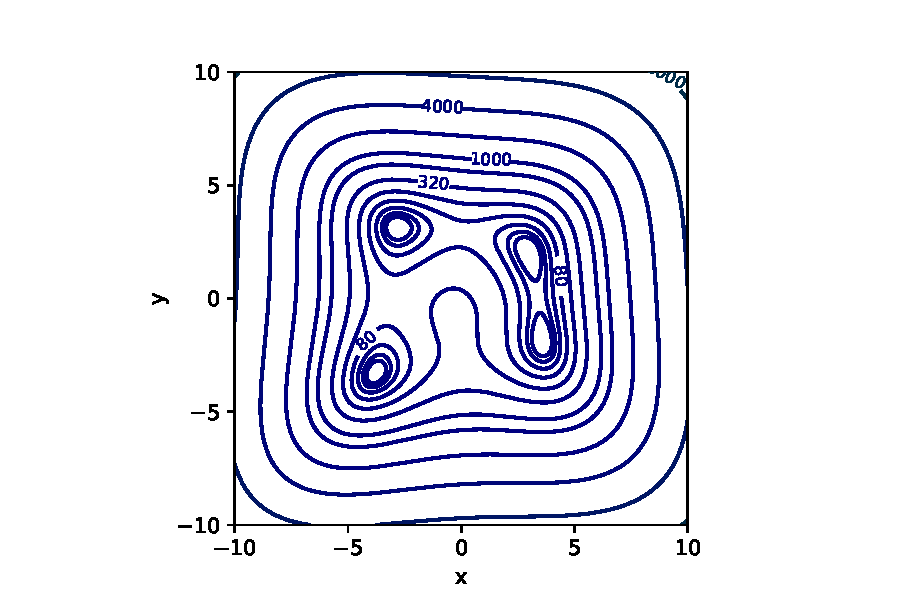
\includegraphics[width=0.35\linewidth]{himmelblau} \\
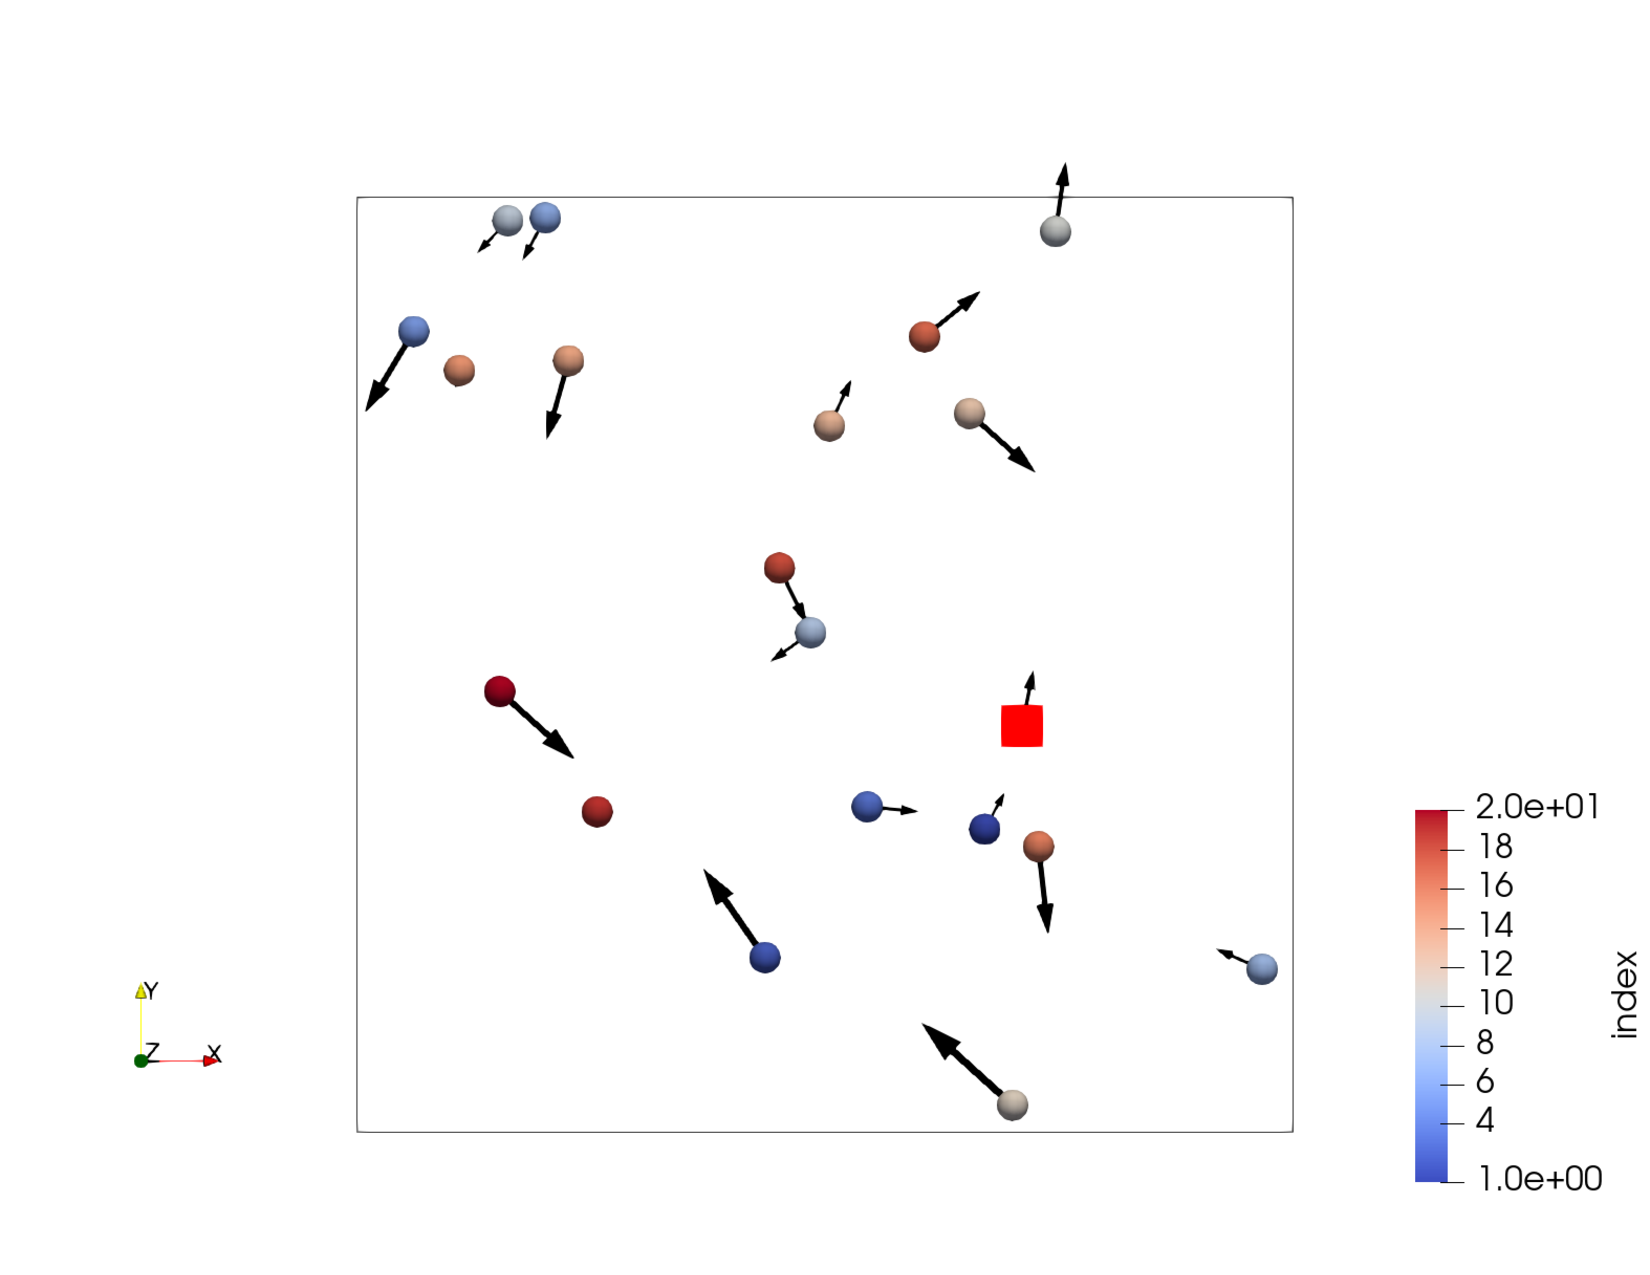
\includegraphics[width=0.3\linewidth]{PSO_animation0}
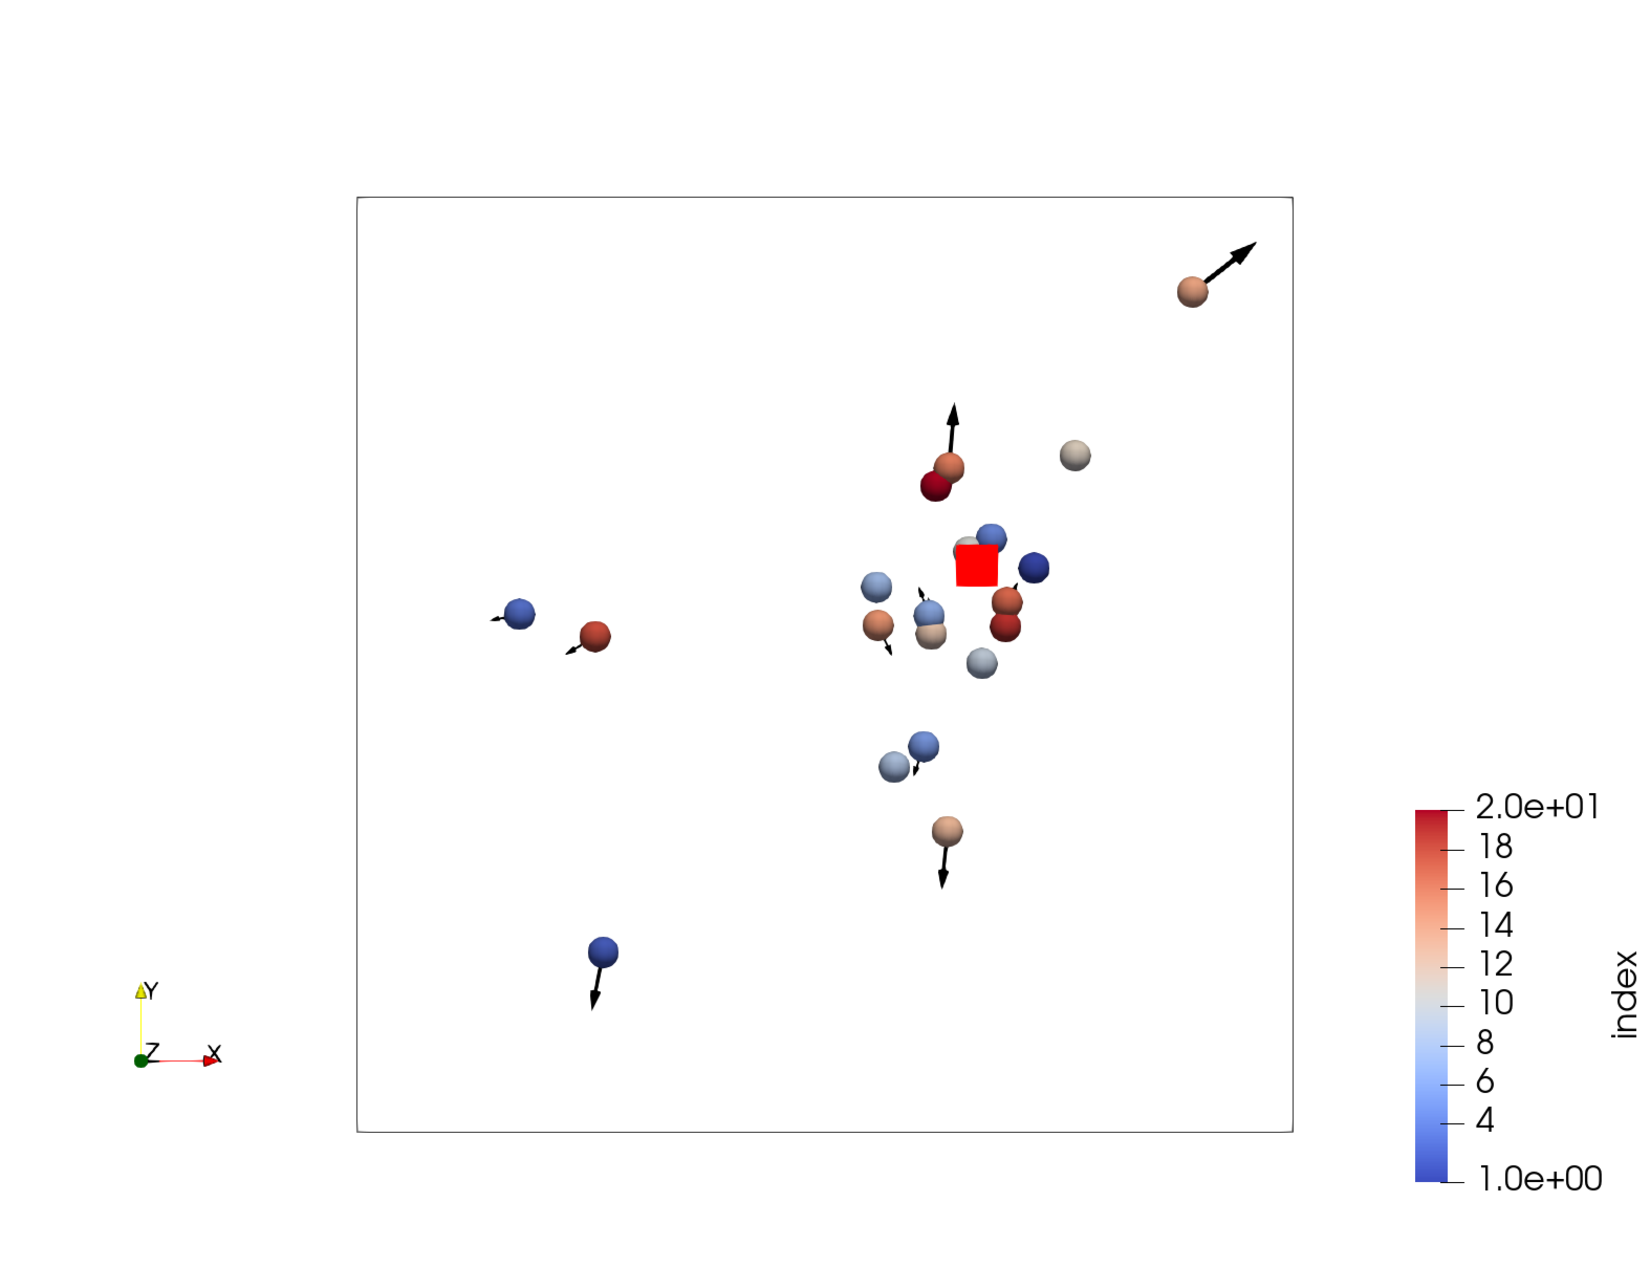
\includegraphics[width=0.3\linewidth]{PSO_animation10}
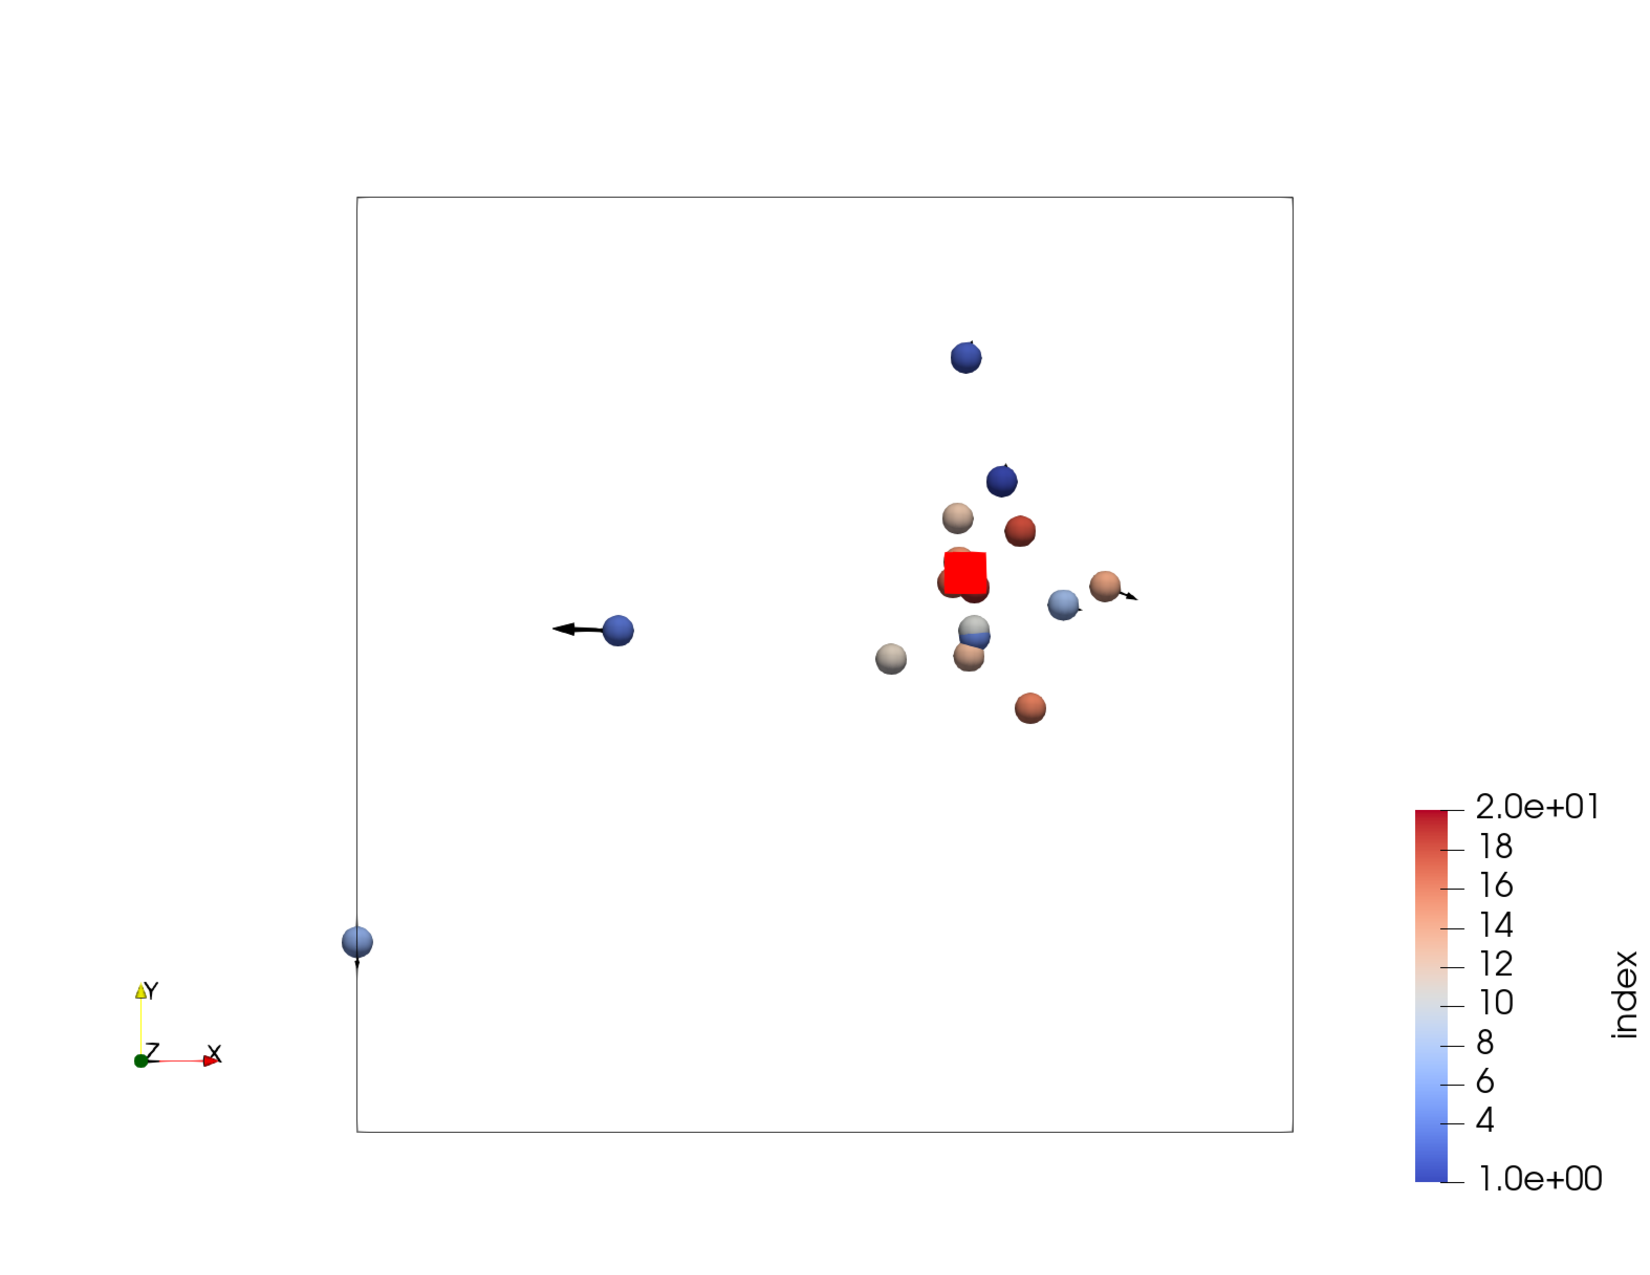
\includegraphics[width=0.3\linewidth]{PSO_animation25}

\caption{Top row: Himmelblau's function has 4 identical local minima shown in contour plots. Bottom row: schematics of finding one of the local minima of Himmelblau's function (top right one in contour plots, see red square in bottom figures which is the global best particle/solution) using Particle Swarm Optimization in 25 iterations (\Np\ = 20, \Niter\ = 0, 10, 25 from left to right, bounds are [-10,10] for both dimensions).}
\label{fig: himmelblau}
\end{figure*}


\subsection{Parallel implementation}
\label{sec: implementation}
PSO is similar to Nbody problem in terms of general implementation.
However, the complexity of one iteration (update) is $O(n)$ instead of $O(n^2)$ because each particle update (location and velocity) is not dependent on the whole population but only based on the global best particle (smallest historical fitness in the group).
One can understand PSO as a simpler version of Nbody problem.
\medskip

\noindent\textbf{OpenMP threading}
Particles (location and velocity) are stored in arrays (\Ndim x \Np).
The implementation updates each particle in OpenMP \emph{for} directive.
OpenMP can ``spawn'' multiple threads to accelerate these loop with \code{\#pragma omp parallel for}.
Because the computation load is more or less the same for calculating each particle, \code{schedule(static)} is used for managing load balance among different threads \cite{eijkhout_2016, eijkhout_2016_2}.

OpenMP threading should be avoided when updating the global best particle because shared memory access could cause a racing condition that leads to false sharing of the global best particle.
There might be some ways to take care of this situation using OpenMP, but they are not considered in the present work. 
\medskip


\noindent\textbf{``Domain decomposition'' with MPI}
The concept analogous to domain decompositions in molecular dynamics and Nbody problem \cite{eijkhout_2016, Bindel_2010} is used in PSO MPI implementation.
The idea is to let each rank (processor) only work on a subgroup (equal amount if possible for load balancing among processors) of the total particle population within each iteration.
After all processors finish their work, the newly updated information is collected and broadcast to all processors before the next iteration with \code{MPI\_Allgather} command.
To ensure synchronization, the update of global best location is done by the master rank and is broadcast to all the other ranks before the next iteration.
\medskip


\subsection{HDF5 I/O}
Due to the high volume of spatial data, HDF5 is the preferred output method to keep track of particle locations and velocities for each iteration. 
The fitness for each iteration and average time cost (total) are printed in the terminal. 


\section{Verification with Himmelblau's function}

Himmelblau's function is a simple two-dimensional function often used to test mathematical optimization algorithms.
Himmelblau's function \cite{Himmelblau_1972} is defined by \cref{eq: himmelblau}.
It has four identical local minima ($f(\cdot)=0$) or ``solutions''.
They are listed in \cref{tab: local_minima} and can be visualized as four concentric circles in the contour plots in \cref{fig: himmelblau}. 

\begin{equation}
f(x,y) = (x^2 + y -11)^2 + (x + y^2 - 7)^2
\label{eq: himmelblau}
\end{equation} 

Subfigures in the bottom row in \cref{fig: himmelblau} demonstrate how 20 PSO particles find one of the correct solutions (red square, the global best particle) in 25 iterations. 
With Himmelblau's function, PSO implementation with either OpenMP or MPI is verified by checking the optimized results with the correct solutions. 
\Cref{tab: local_minima} also shows the optimized results by PSO with OpenMP.
It usually takes a few hundred iterations to find solutions whose fitness $<$ 0.05  (less than a \SI{5}{\percent} deviation compared to the correct minima).

\begin{table}[h!]
\captionof{table}{Four local minima of Himmelblau's function and the optimized results by PSO with OpenMP (fitness $<$ 0.05, bounds are [-20, 20] for both dimensions). }
\label{tab: local_minima}
\begin{center}
\begin{tabular}{ cccc } 
\toprule
minima (x,y) & omp optimized (x,y) & iterations & fitness \\
 \midrule
 \num{3.0}, \num{2.0} &\num{2.966499}, \num{2.038675} & 301& \num{0.041042}\\
 \num{-2.805118}, \num{3.131312}  &\num{-2.835503}, \num{3.123740 }& 140& \num{0.032881}\\
 \num{-3.779310}, \num{-3.283186} &\num{-3.762330}, \num{-3.256691}  & 307&\num{0.034743}\\
 \num{3.584428}, \num{-1.848126} &\num{3.574093}, \num{-1.797977} &  131& \num{0.037889} \\
 \bottomrule
\end{tabular}
\end{center}
\end{table}


\section{Results and discussions}
In order to compare the performance of different parallel strategies, a fixed iteration number (\Niter=100) is used for all cases.
To minimize fluctuations, the averaged time cost of 10 repetitive runs is used as the metric.

Strong scaling and weak scaling studies are done for both parallel methods.
Strong scaling studies the speedup of a fixed-size problem with varying processor numbers, which is governed by Amdahl's law.
In comparison, weak scaling investigates a scaled size problem with a fixed workload per processor and obeying Gustafson's law \cite{eijkhout_2016, eijkhout_2016_2}.
The efficiency of strong scaling $E_\text{strong}$ and weak scaling $E_\text{weak}$ are calculated in \cref{eq: strong_scaling} and \cref{eq: weak_scaling}.
Both $E_\text{strong}$ and $E_\text{weak}$ are expected to follow an asymptotic decay due to increasing overhead cost with more processor/threads used.

\begin{align}
E_\text{strong} &= \frac{T_1}{\text{\Nproc}\times T_n}  
\label{eq: strong_scaling}\\
E_\text{weak} &= \frac{T_1}{T_n}
\label{eq: weak_scaling}
\end{align}

All jobs are submitted on Intel18-dev node on ICER High Performance Computing clusters at Michigan State University.



\subsection{Strong scaling of OpenMP implementation (thread-to-thread speedup)}

\Np=100, 8000, and 16000 are fixed for \code{OMP\_NUM\_THREADS}=1, 2, 4, 8, 16, 32, and 40 respectively.
The performance are plotted in \cref{fig: omp_strong}.
For \Np=100 and 8000, the time cost slightly increases with more threads spawned.
This is because the fitness calculations (Himmelblau's function) are small, so the overhead cost from spawning more threads time outweighs the cost saved by parallel executions. 
When \Np\ is increased to 16000, the time cost starts to slightly decrease with more threads.
Unfortunately, \Np=16000 is the max particle number the default memory could handle, so it could not be tested further.
It is expected to see time cost would reduce more significantly with increasing thread numbers for \Np $>$ 16000.

The efficiency of every \Np\ follows an asymptotic decay, which is expected.

\begin{figure}[h!]
\centering
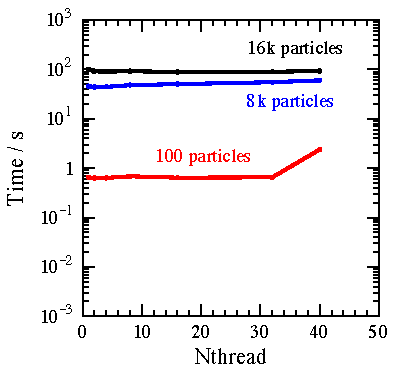
\includegraphics[width=0.45\linewidth]{omp_strong_time} 
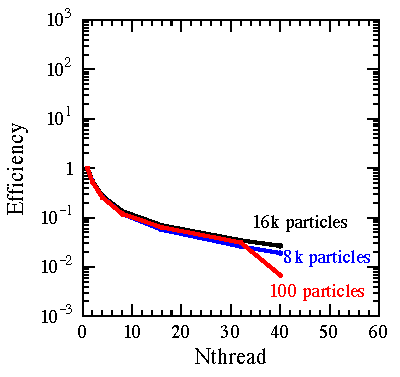
\includegraphics[width=0.45\linewidth]{omp_strong_effi}
\caption{Strong scaling study of OpenMP PSO for \Np=100, 8000, and 16000 (max particles default memory can handle).}
\label{fig: omp_strong}
\end{figure}

\subsection{Weak scaling of OpenMP implementation}

Since PSO has $O(n)$ complexity, a linear scale-up of \Np\ with \Nthreads\ is used to maintain the local workload at 400 and 1000 particles/thread, respectively.
In an ideal scenario (no extra cost associated with spawning threads), if the problem is perfectly parallelizable, a flat line (time cost) is expected to see.
However, \cref{fig: omp_weak} shows a significant overhead cost associated with spawning more threads compared to the actual calculation cost such that the time cost increases with more threads (efficiency decreases) for this problem.
On the other hand, efficiency also drops asymptotically with increasing thread number.

\begin{figure}[h!]
\centering
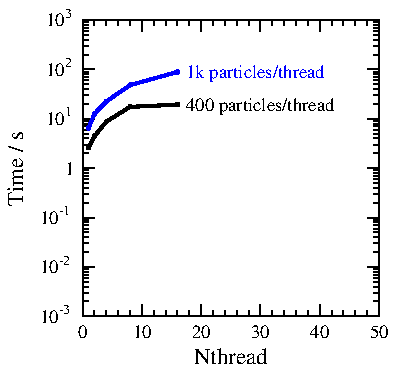
\includegraphics[width=0.45\linewidth]{omp_weak_time} 
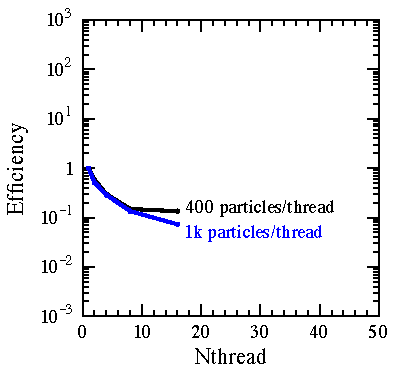
\includegraphics[width=0.45\linewidth]{omp_weak_effi}
\caption{Weak scaling study of OpenMP PSO for work load of 400 and 1000 particles per thread.}
\label{fig: omp_weak}
\end{figure}


\subsection{Strong and weak scaling of MPI implementation}
 Despite the MPI code can get the correct solutions for \Nproc=2, it cannot run when $\Nproc > 2$ for some reasons (return segmentation 11 error). 
This may due to the way memory is allocated in the present implementation.
Therefore, I can only show results  for \Nproc=1, 2 and up to \Np=1000 (max particles for MPI implementation).
Due to the limited data points, not much generalization can be made about the performance except two take-aways: (a) time cost increases a lot as \Nproc\ increases to 2; (b) MPI implementation has arguably more time cost compared to OpenMP for both strong and weak scaling studies.
This might be MPI implementation has a lot more cost associated with communication (\code{MPI\_Bcast} and \code{MPI\_Allgathter} among all processors) compared to OpenMp thread spawning.


\begin{figure}[h!]
\centering
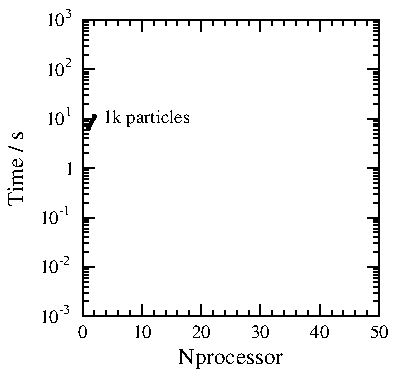
\includegraphics[width=0.45\linewidth]{mpi_strong_time} 
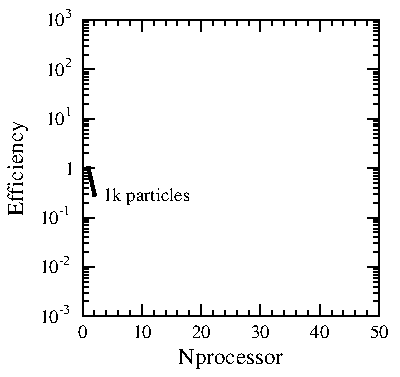
\includegraphics[width=0.45\linewidth]{mpi_strong_effi} \\
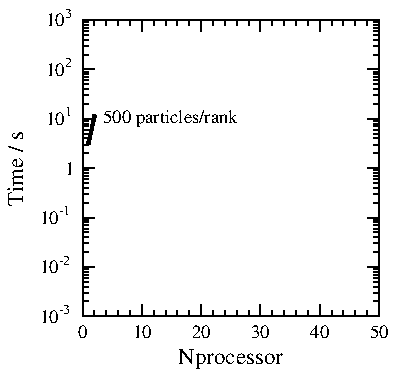
\includegraphics[width=0.45\linewidth]{mpi_weak_time} 
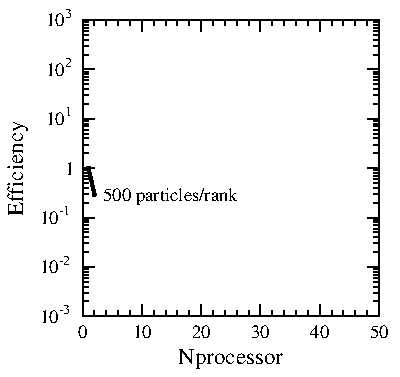
\includegraphics[width=0.45\linewidth]{mpi_weak_effi}
\caption{Strong (top row) and weak (bottom) scaling study with MPI.}
\label{fig: mpi_scaling}
\end{figure}


\subsection{Load balancing}
As is discussed in \cref{sec: implementation}, \code{\#pragma parallel omp for schedule(static)} is used to ensure every thread has more or less the same workload during OpenMP threading.
Since the cost to calculate the fitness value for each particle update is almost the same, an equal number of particles are distributed to each processor in MPI parallelization to balance the workload among processors.

\subsection{Memory usage}
In the sequential implementation, all variables are defined as global variables to ensure it does not need to duplicate data when updating particles.
However, the max particle number it could handle (with default memory) is \Np=16000.
More memory could be requested through Slurm to allow more particle numbers.

For OpenMP implementation, memory is not a big issue as threads use shared memory.
MPI implementation would have more memory limitation because each processor needs to duplicate the entire dataset, and the memory burden scales up with \Nproc\ (max \Np=1000 for MPI implementation).
A future improvement to address this issue is to pass data only relating to the particle subgroup to each processor. 


\section{Summary}
Parallel computing implementation of particle swarm optimization (PSO) was developed with OpenMP and MPI, respectively.
The speedup performance of both parallel methods was evaluated by comparing it with that of a sequential implementation in both strong and weak scaling studies. 
The performance did not show a significant speedup for both parallel methods.
This indicates PSO is not complicated enough (when fitness calculation is also cheap) to use either parallel scheme (OpenMP or MPI). 
A hybrid parallel paradigm (OpenMP + MPI) needs further investigation.
However, when the fitness calculation requires enormous efforts (such as finite element modeling), parallel computing is expected to have considerable speedup.  
It would also be interesting to test this in future practice.


\section*{Acknowledgement}
This is a term report for the parallel computing course offered by the Department of Computational Mathematics, Science, and Engineering, at Michigan State University. 
The author greatly appreciates the inspiration and help from professor Sean M. Couch.
The computational calculation of this work was supported by ICER High Performance Computing Clusters (HPCC) at Michigan State University.

\section*{Code availability}
The source codes can be found at \href{https://github.com/zhuowenzhao/particle_swarm_parallel_implementation}{\nolinkurl{https://github.com/zhuowenzhao/particle_swarm_parallel_implementation}}.

\bibliographystyle{IEEEtrans}
\bibliography{pso}

\end{document}
